% This is "sig-alternate.tex" V2.0 May 2012
% This file should be compiled with V2.5 of "sig-alternate.cls" May 2012
%
% This example file demonstrates the use of the 'sig-alternate.cls'
% V2.5 LaTeX2e document class file. It is for those submitting
% articles to ACM Conference Proceedings WHO DO NOT WISH TO
% STRICTLY ADHERE TO THE SIGS (PUBS-BOARD-ENDORSED) STYLE.
% The 'sig-alternate.cls' file will produce a similar-looking,
% albeit, 'tighter' paper resulting in, invariably, fewer pages.
%
% ----------------------------------------------------------------------------------------------------------------
% This .tex file (and associated .cls V2.5) produces:
%       1) The Permission Statement
%       2) The Conference (location) Info information
%       3) The Copyright Line with ACM data
%       4) NO page numbers
%
% as against the acm_proc_article-sp.cls file which
% DOES NOT produce 1) thru' 3) above.
%
% Using 'sig-alternate.cls' you have control, however, from within
% the source .tex file, over both the CopyrightYear
% (defaulted to 200X) and the ACM Copyright Data
% (defaulted to X-XXXXX-XX-X/XX/XX).
% e.g.
% \CopyrightYear{2007} will cause 2007 to appear in the copyright line.
% \crdata{0-12345-67-8/90/12} will cause 0-12345-67-8/90/12 to appear in the copyright line.
%
% ---------------------------------------------------------------------------------------------------------------
% This .tex source is an example which *does* use
% the .bib file (from which the .bbl file % is produced).
% REMEMBER HOWEVER: After having produced the .bbl file,
% and prior to final submission, you *NEED* to 'insert'
% your .bbl file into your source .tex file so as to provide
% ONE 'self-contained' source file.
%
% ================= IF YOU HAVE QUESTIONS =======================
% Questions regarding the SIGS styles, SIGS policies and
% procedures, Conferences etc. should be sent to
% Adrienne Griscti (griscti@acm.org)
%
% Technical questions _only_ to
% Gerald Murray (murray@hq.acm.org)
% ===============================================================
%
% For tracking purposes - this is V2.0 - May 2012

\documentclass{sig-alternate}

\usepackage{listings,xcolor,bera}
\usepackage{graphicx}
%% \usepackage{afterpage}

\colorlet{punct}{red!60!black}
\definecolor{background}{HTML}{EEEEEE}
\definecolor{delim}{RGB}{20,105,176}
\colorlet{numb}{magenta!60!black}

\lstdefinelanguage{json}{
    basicstyle=\normalfont\ttfamily,
    numbers=left,
    numberstyle=\scriptsize,
    stepnumber=1,
    numbersep=8pt,
    showstringspaces=false,
    breaklines=true,
    frame=lines,
    %% backgroundcolor=\color{background},
    literate=
     *{0}{{{\color{numb}0}}}{1}
      {1}{{{\color{numb}1}}}{1}
      {2}{{{\color{numb}2}}}{1}
      {3}{{{\color{numb}3}}}{1}
      {4}{{{\color{numb}4}}}{1}
      {5}{{{\color{numb}5}}}{1}
      {6}{{{\color{numb}6}}}{1}
      {7}{{{\color{numb}7}}}{1}
      {8}{{{\color{numb}8}}}{1}
      {9}{{{\color{numb}9}}}{1}
      {:}{{{\color{punct}{:}}}}{1}
      {,}{{{\color{punct}{,}}}}{1}
      {\{}{{{\color{delim}{\{}}}}{1}
      {\}}{{{\color{delim}{\}}}}}{1}
      {[}{{{\color{delim}{[}}}}{1}
      {]}{{{\color{delim}{]}}}}{1},
}

\begin{document}

\makeatletter
\def\@copyrightspace{\relax}
\makeatother


\title{
Duck - Yet Another Sofware Visualization Tool to Speed Up Source Codes Understanding
}

\numberofauthors{5} %  in this sample file, there are a *total*
% of EIGHT authors. SIX appear on the 'first-page' (for formatting
% reasons) and the remaining two appear in the \additionalauthors section.
%
\author{
% You can go ahead and credit any number of authors here,
% e.g. one 'row of three' or two rows (consisting of one row of three
% and a second row of one, two or three).
%
% The command \alignauthor (no curly braces needed) should
% precede each author name, affiliation/snail-mail address and
% e-mail address. Additionally, tag each line of
% affiliation/address with \affaddr, and tag the
% e-mail address with \email.
%
% 1st. author
\alignauthor
Shan He\\
       \affaddr{504774265}\\
       \email{shanhex@gmail.com}
% 2st. author
\alignauthor
Yukai Tu\\
       \affaddr{204761085}\\
       \email{tuyukai1994@gmail.com}
% 3st. author
\alignauthor
Yuling Liu\\
       \affaddr{504777221}\\
       \email{lylwill@umich.edu}
\and
% 4st. author
\alignauthor
Yumin Xia\\
       \affaddr{404775675}\\
       \email{yumin@cs.ucla.edu}
% 5st. author
\alignauthor
Cong Peng\\
       \affaddr{904760493}\\
       \email{pengcong@ucla.edu}
}

\maketitle
\begin{abstract}
This paper is the proposal of a language independent, interactive, software visualization analysis tool called Duck, which supports presenting polymetric views of source code, based on syntactical and runtime statistics, that could be processed by data mining algorithms.
\end{abstract}

\section{Motivation}

Nowadays, as codebases grow larger, software systems are one of the most complex and difficult systems to understand.
Meanwhile, reading source codes and understanding key modules are time-consuming prerequisites for the followed software development.
To speed up this process, software visualization technique is proposed to be an efficient technique
to facilitate source code understanding, because visual displays allow the human brain to study
multiple aspects of complex problems in parallel \cite{petre1995looking}.
Also, developers can form an initial mental picture of the system through visualized diagram \cite{lanza2003object}
and even veteran programmers find it useful \cite{kim2012field}. 

However, visualization technique has downsides.
For example, they are usually measured in a single degree,
hard to scale up and lack of visual cues for the viewer to correctly interpret them \cite{fenton2014software}.
To overcome the single degree measurement, \cite{lanza2003polymetric} presents a visual approach that captures multiple software metrics,
like lines of code, method overridden ratio and number of state variable etc.,
linked up associatively, in a single diagram,
to help to understand the structure in an initial phase.
As an enhancement of \cite{lanza2003polymetric}, we plan to combine following innovations into polymetric view \cite{lanza2003polymetric}:

\begin{enumerate}
  \item Combining runtime statistics, i.e. program profile, with syntactic metrics. For example, user can pass a profile of a program against a specific input, alone with the source code, the execution time metrics and static metrics will be drawn on the output diagrams, associatively. We hope that, by this way, there will be more clear cues for viewer to interpret the figures.
  \item Application of data mining techniques on metrics. For example, by applying the PageRank algorithm on function call graphs, we can evaluate the importance of functions.
  \item Visualization query to selectively show limited classes or methods that user cares. This query could also make visualization more scalable.
\end{enumerate}

To summarize, we propose a language independent, interactive, software visualization analysis tool called Duck, which supports presenting polymetric views of source code, based on syntactical and runtime statistics, that could be processed by data mining algorithms.

\section{Related Work}
When developers who first look at an unfamiliar code base,
it is usually hard to get an overall picture of the whole system.
\cite{stasko1998software} presents some basic ideas on how to build a mental model during software exploration,
but do not provide the much-needed, yet difficult to obtain, empirical evidence.
Lanza, M., and Ducasse, S in \cite{lanza2003polymetric} settled on the following goals for getting a first impression and a mental model of a system:

\begin{enumerate}
\item code base size, complexity, structure.
\item understand the most important classes and inheritance hierarchies.
\item Identify exceptional classes in terms of size and/or complexity.
\item Identify the possible presence of design patterns.
\end{enumerate}

To get above information from a code base, in the wide array of possible metrics,
we plan to selected the design metrics, which can be extracted from the source code entities themselves.
The metrics we use are termed direct measurement metrics, also include parts of indirect measurement \cite{storey1999cognitive}.

Since software visualizations are often too simplistic and lack visual cues for the viewer to correctly interpret them \cite{petre1995looking},
the most common way is to increase the dimension of the graphs, like concretization and polymetric.
Not only increase the dimension from 2D to 3D, the Codecity also concretize a code base into a city model \cite{wettel2008codecity}.
The buildings in the city represent classes, while the districts represent the software packages.
The CodeCity supports both linear mapping and non-linear mapping for metrics and uses containment-based layout to
display the nesting level of package in each district. In another way, the polymetric try
to present multiple corresponding information within different polymetric layouts \cite{lanza2003polymetric, lanza2005codecrawler, lanza2003object}.
In \cite{lanza2003object}, page 21, it defines the layout types include: Tree, Scatterplot, Histogram, Checker, Stapled, etc.
An implementation of this visualization tool can be found at this website \footnote{http://www.softviscollection.org/polymetric-views/public/polymetrics.html},
which can generate 6 layouts graph in real-time. 

In our project, we not only re-implement the previous work, but also improve the metrics and visualization result.
In metrics, we try to introduce the dynamic supervision on variables, methods, and classes runtime behavior.
In visualization output, we hope a more intuitive, more efficient graphical representation can be achieved.

\section{Approach Description}

\begin{figure*}
\centering
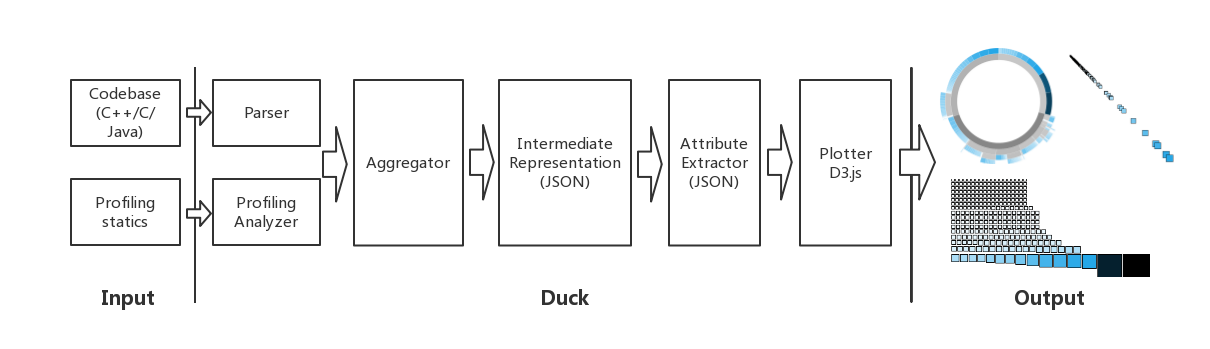
\includegraphics[width=1.0\textwidth]{arch.png}
\caption{Architecture of Duck}
\label{fig:arch}
\end{figure*}

To implement this tool, we use a layered architecture, shown in Figure \ref{fig:arch}. Our program will include the following modules:

\begin{enumerate}
\item Parser and Profiling Analyzer
\item The Aggregator module 
\item Intermediate representation module
\item Attribute Extractor
\item Plotter D3.js
\end{enumerate}

For the input, the user need to specify the code base location.
The Duck will be a language independent visualization tool so the language may include C++, C, Java, etc.
User also need to assign the profiling statics to the Duck.

The first layer of Duck is a language-dependent parser and a compiler-dependent profiling statics analyzer.
In this project, we plan to at least implement supports for C++11 and its profile,
based on Clang parser libraries and using GNU/Linux’s gcc profiling tool GPROF to sample runtime statistics.

The second layer, Aggregator, is designed to combine inputs from parser and profiling
analyzer to generate an intermediate representation(IR). The IR module is a library of
classes that takes the input from the Aggregator and provides functions of querying statics,
used by AttributeExtractor. This module also hides the changes of concrete representation implementation: currently,
we plan to use json format as storage format. An example of IR can be found at appendix \ref{IReg}. 

The AttributeExtractor extracts interesting metrics from IR, and passing those metrics to plotter.
The plotter module is based on a javascript library D3.js and reuses some codes
from a previous polymetric view implementation\footnote{https://github.com/softvis/polymetric-views}.
Thus, Plotter will draw interative diagram on browser.

\section{Evaluation Plan}
We will invite two groups of people (Namely, group A and group B) to read a code base,
which is totally new to them. We will provide people in group A with our visualization
tool as a helper. After both groups read the code base, we will send out our survey on
how much do they understand the code base.
The survey includes some questions such as 1. What is the hierarchy between certain functions?
2. What is the top-down structure of the code base, and to what extent do they think they understand the system?
After collecting a reasonable amount of survey results, experienced developers, who are
already familiar with the code, will then evaluate the understanding level towards the code base
between these two groups by analyzing their answers. Hopefully, the result can tell to what extent does
our visualization helper helps people understanding a brand new code base.

To further evaluate the Duck with previous visualization tool,
we will also conduct the same experiment and two groups will equipped with Duck and other visualization tool, like [10].
We hope the differences between these tool can be demonstrated by the survey and hopefully, Duck will get a higher score.

\begin{figure}
\centering
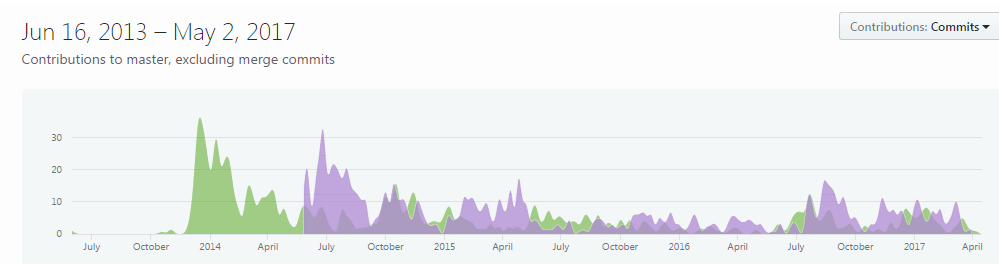
\includegraphics[scale=.243]{ndn.png}
\caption{NFD(purple) and ndn-cxx(green) contribution history}
\label{fig:ndn}
\end{figure}

The tested code bases will be Named-Data Networking (NDN) projects\cite{ndn}: NDN Forwarding Daemon (NFD), and ndn-cxx, NDN C++ library (shown in Figure \ref{fig:ndn}).
Both code bases are 3-year-old,
well structured and well defined. More than 30 members have participated and more than thousands of detailed code review commits were committed.
Both projects are implemented in C++ and more than 60000 lines of code.
These code bases are in perfect size which needs programmer spend some time on getting a whole picture of the project.
The managers of these projects are professors and doctoral students in Internet Research Lab, UCLA, who can
provide the feedbacks after we collect the survey.


%% \footnote{This is the second footnote.  It
%% starts a series of three footnotes that add nothing
%% informational, but just give an idea of how footnotes work
%% and look. It is a wordy one, just so you see
%% how a longish one plays out.}

%% \cite{Lamport:LaTeX}

%
% The following two commands are all you need in the
% initial runs of your .tex file to
% produce the bibliography for the citations in your paper.
\bibliographystyle{abbrv}
\bibliography{sigproc}  % sigproc.bib is the name of the Bibliography in this case
% You must have a proper ".bib" file
%  and remember to run:
% latex bibtex latex latex
% to resolve all references
%
% ACM needs 'a single self-contained file'!
%
%APPENDICES are optional
%\balancecolumns
\appendix
%Appendix A
\section{Intermediate Representation Example}
\label{IReg}

\begin{lstlisting}[language=json,firstnumber=1]
{  
   "classes":{  
      "foo":{  
         "inherited list":[  
            "BaseA",
            "BaseB"
         ],
         "methods":[  
            {  
               "addAandB":{  
                  "parameter":[  
                     { "xx":"Int"   },
                     { "yy":"Bool"  },
                     { "zz":"String }
                  ],
                  "calling-function":[  
                     "Bar.subAandB",
                     "Pc.test"
                  ],
                  "linesOfCode":38,
                  "run-time invokes":10
               }
            }
         ]
      }
   }
}
\end{lstlisting}

\end{document}
